\chapter{Tutorial Python}\label{ap:python}
\section{Introdução}
\begin{itemize}
	\item Linguagem aberta, gratuita e de fácil aprendizado
	\item Linguagem de programação de alto nível (a programação é com palavras comuns da língua inglês, como \textit{print} para \textit{exibir} na tela)
	\item O uso no curso pode ser instalando o próprio pacote oficial do Python, instalando o Anaconda (um conjunto de ferramentas para processamento científico) ou usando o Google Colaboratory
	\item O \textit{Python} é uma linguagem interpretativa, significando que não é necessária a compilação para seu uso (não é necessário converter previamente o código para linguagem de máquina, como em outras linguagens). O interpretador do \textit{Python} pode ser executado interativamente, o que é útil para testar em tempo real a linguagem. Neste texto, códigos começados por \verb|>>>| são escritas diretamente no interpretador, e não em um arquivo de texto, e as linhas seguintes sem o \verb|>>>| são a resposta do comando executado. Linhas de continuação são representadas por \verb|...| e aparecem em construções de várias linhas, sempre endentadas (com um recuo, geralmente de 4 espaços em branco):
	\begin{minted}{python}
>>> print("Olá, mundo.")
Olá, mundo.
>>> if True:
...     print("Multi-linhas sempre precisam de endentação.")
... 
Multi-linhas sempre precisam de endentação.
	\end{minted}
\end{itemize}

\section{Comandos básicos}
\begin{itemize}
	\item Atribuições são feitas utilizando \verb|=| e comentários usando \verb|#|
	\begin{minted}{python}
# primeiro comentário
spam = 1  # segundo comentário
# um terceiro comentário
texto = "# este não é um comentário, pois está entre aspas."
	\end{minted}
	\item O interpretador funciona como uma simples calculadora, com os símbolos padrão funcionando para a maioria dos operadores:
	\begin{minted}{python}
>>> 2 + 2
4
>>> 50 - 5*6
20
>>> (50 - 5*6) / 4
5.0
>>> 8 / 5  # divisão sempre retorna um número em ponto flutuante (não inteiro)
1.6
	\end{minted}
	\item Para descartar a parte fracionária da divisão usa-se \verb|//| e \verb|%| para calcular o resto da divisão
	\begin{minted}{python}
>>> 17 / 3  # divisão clássica retorna ponto flutuante
5.666666666666667
>>>
>>> 17 // 3  # descarta a parte fracionária
5
>>> 17 % 3  # retorna o resto da divisão
2
>>> 5 * 3 + 2  # quociente * divisor + resto
17
	\end{minted}
	\item Usa-se \verb|**| para calcular potências
	\begin{minted}{python}
>>> 5 ** 2  # 5 ao quadrado
25
>>> 2 ** 7  # 2 elevado a 7
128
	\end{minted}
	\item Nenhum resultado é exibido ao fazer atribuições a uma variável
	\begin{minted}{python}
>>> largura = 20
>>> altura = 5 * 9
>>> largura * altura
900
	\end{minted}
\end{itemize}

\section{Sequências de texto (\textit{strings})}
\begin{itemize}
	\item Sequências de texto podem ser definidas entre aspas simples (\verb|'...'|) ou duplas (\verb|"..."|) com o mesmo resultado, e o caractere \verb|\| é usado para escapar as aspas (considerá-las como parte do texto, e não o marcador de fim da \textit{string}):
	\begin{minted}{python}
>>> 'ovo frito'  # aspas simples
'ovo frito'
>>> 'McDonald\'s' # usando \' para escapar a aspa simples
"McDonald's"
>>> "McDonald's"  # ... ou use aspas duplas
"McDonald's"
>>> '"Sim", eles disseram.'
'"Sim", eles disseram.'
>>> "\"Sim\", eles disseram."
'"Sim", eles disseram.'
	\end{minted}
	\item \textit{Strings} podem ser concatenadas (juntadas) usando o operador \verb|+|, e repetidas com \verb|*|
	\begin{minted}{python}
>>> # 'a' seguido de 'ra' duas vezes
>>> 'a' + 2 * 'ra'
'arara'
	\end{minted}
	\item \textit{Strings} podem ser indexadas, com o primeiro caractere tendo índice 0, e pode-se utilizar índices negativos, para contar da direita para a esquerda
	\begin{minted}{python}
>>> palavra = 'Python'
>>> palavra[0]  # caractere na posição 0
'P'
>>> palavra[5]  # caractere na posição 5
'n'
>>> palavra[-1]  # último caractere
'n'
>>> palavra[-2]  # penúltimo caractere
'o'
>>> palavra[-6]
'P'
	\end{minted}
	\item O fatiamento (\textit{slicing}) também é suportado. Enquanto a indexação é usado para o acesso a um único caractere, o fatiamento permite a obtenção de sub-sequências. O começo sempre é incluído, enquanto o final é sempre excluído, o que garante que \verb|s[:i] + s[i:]| é sempre igual à \verb|s|
	\begin{minted}{python}
>>> palavra[0:2]  # caractere da posição 0 (incluído) até 2 (excluído)
'Py'
>>> palavra[2:5]  # caractere da posição 2 (incluído) até 5 (excluído)
'tho'
>>> palavra[:2] + palavra[2:]
'Python'
>>> palavra[:4] + palavra[4:]
'Python'
	\end{minted}
	\item Os índices de fatiamento possuem alguns padrões úteis: a omissão do primeiro item tem 0 como padrão, enquanto que a omissão do segundo tem como padrão o comprimento da \textit{string}
	\begin{minted}{python}
>>> palavra[:2]  # caracteres do começo até a posição 2 (excluído)
'Py'
>>> palavra[4:]  # caracteres da posição 4 (incluído) até o final
'on'
>>> palavra[-2:]  # caracteres da penúltima posição (incluído) até o final
'on'
	\end{minted}
	\item A função \verb|len()| retorna o comprimento da string
	\begin{minted}{python}
>>> s = 'supercalifragilisticexpialidocious'
>>> len(s)
34
	\end{minted}
\end{itemize}

\section{Estruturas de controle de fluxo}
\begin{description}
	\item[enquanto (\textit{while})] Repete uma sequência de ações enquanto a condição for verdadeira
	\begin{minted}{python}
>>> # Sequência de Fibonacci:
... # a soma de dois elementos define o próximo
... a, b = 0, 1  # atribuição múltipla (a recebe 0, b recebe 1)
>>> while a < 10:  # a condição é o valor de a ser menor que 10
...     print(a)
...     a, b = b, a+b
...
0
1
1
2
3
5
8
	\end{minted}
	\item[se (\textit{if})] Executa uma ação se a condição for verdadeira. Pode ter inúmeras outras condições caso a primeira seja falsa (comando \verb|elif|) e uma caso todas sejam falsas (comando \verb|else|)
	\begin{minted}{python}
>>> x = int(input("Por favor, digite um inteiro: "))
Por favor, digite um inteiro: 42
>>> if x < 0:
...     x =  0
...     print('Valor negativo alterado para zero')
... elif x == 0:
...     print('Zero')
... elif x == 1:
...     print('Unitário')
... else:
...     print('Mais')
... 
Mais
	\end{minted}
	\item[para (\textit{for})] Itera ao longo dos itens de uma sequência
	\begin{minted}{python}
>>> # Mede algumas strings:
>>> palavras = ['gato', 'janela', 'marmota']
>>> for palavra in palavras:
...    print(palavra, len(palavra))
... 
gato 4
janela 6
marmota 7
	\end{minted}
	\item[faixa (\textit{range})] Gera progressões aritméticas. É útil para iterar ao longo de uma sequência de números. Os argumentos são, na ordem, \textbf{início} (primeiro valor da sequência, inclusivo), \textbf{fim} (valor final da sequência, exclusivo) e \textbf{passo} (de quanto em quanto os valores são contados). Caso tenha apenas dois argumentos, assume que o passo é 1, e caso só tenha um argumento, assume que o primeiro valor é 0
	\begin{minted}{python}
>>> for i in range(5):
...     print(i)
...
0
1
2
3
4
"""
range(5, 10)
5, 6, 7, 8, 9

range(0, 10, 3)
0, 3, 6, 9

range(-10, -100, -30)
-10, -40, -70
"""
	\end{minted}
\end{description}

\section{Funções}
\begin{itemize}
	\item Funções em \textit{Python} são definidas pela palavra-chave \verb|def|, seguida do nome da função e a lista de parâmetros entre parêntesis
	\item Todas as definições dentro da função precisam estar endentadas
	\item A primeira linha de definição pode ser uma sequência de texto, chamada de \textit{docstring}. Se presente, é usada para descrever a função e seu uso \footnote{Mais informações sobre \textit{docstrings} podem ser encontradas na \href{https://docs.python.org/3/tutorial/controlflow.html\#documentation-strings}{documentação online do \textit{Python}} (em inglês)}
	\begin{minted}{python}
>>> def fib(n):    # escreve a sequência de Fibonacci até n
...     """Escreve a sequência de Fibonacci até n."""
...     a, b = 0, 1
...     while a < n:
...         # o 'end' aqui indica que os valores serão separados por espaços
...         # ao invés de separados por linha (o padrão)
...         print(a, end=' ')
...         a, b = b, a+b
...     print()
...
>>> # Agora chama a função que acabou de ser definida:
... fib(2000)
0 1 1 2 3 5 8 13 21 34 55 89 144 233 377 610 987 1597
	\end{minted}
\end{itemize}

\section{Bibliotecas}
\begin{itemize}
	\item Bibliotecas (módulos) no \textit{Python} são importadas usando a sintaxe abaixo:
	\begin{minted}{python}
		import sys
	\end{minted}
	\item Podem ser importadas atribuindo-se um apelido:
	\begin{minted}{python}
		import builtins as bt
	\end{minted}
	\item Funções específicas podem ser importadas diretamente:
	\begin{minted}{python}
		import sound.effects.echo
		# ou
		from sound.effects import echo
	\end{minted}
	\item E também podem ter apelidos:
	\begin{minted}{python}
		import sound.effects.echo as see
		# ou
		from sound.effects import echo as see
	\end{minted}
	\item Todas as funções de um pacote podem ser importadas (não recomendável):
	\begin{minted}{python}
		from sound.effects import *
	\end{minted}
	\item Códigos de outros arquivos podem ser importados como módulos:
	\begin{minted}{python}
		import meu_arquivo
		# ou
		from meu_arquivo import minha_funcao
	\end{minted}
\end{itemize}

\subsection{Numpy}
\begin{itemize}
	\item Biblioteca para processamento matemático
	\item Geralmente é importada usando \mint{python}|import numpy as np|
	\item O elemento base é o vetor (\textit{array}), que possui diversos atributos e métodos associados a ele
	\begin{minted}{python}
>>> a = np.array([2, 3, 4])
>>> a
array([2, 3, 4])
>>> a.shape
(3,)
>>> a.ndim
1
	\end{minted}
	\item É comum não se saber o conteúdo futuro de um vetor, mas o tamanho sim, e por isso existem funções para criar vetores com conteúdos e tamanhos específicos:
	\begin{description}
		\item[zeros] Cria um vetor preenchido com zeros
		\begin{minted}{python}
>>> np.zeros((3,4))
array([[0., 0., 0., 0.],
[0., 0., 0., 0.],
[0., 0., 0., 0.]])
		\end{minted}
		\item[ones] Cria um vetor preenchido com 1
		\begin{minted}{python}
>>> np.ones((2,3))
array([[1., 1., 1.],
[1., 1., 1.]])
		\end{minted}
		\item[empty] Cria um vetor com valores aleatórios extremamente pequenos, obtidos com base no que está presente na memória, e por isso é ligeiramente mais rápido que os anteriores para ser gerado
		\begin{minted}{python}
>>> np.empty((2, 4))
array([[4.67379042e-310, 0.00000000e+000, 6.79038654e-313,
2.22809558e-312],
[2.14321575e-312, 2.46151512e-312, 2.41907520e-312,
5.97819431e-322]])
		\end{minted}
		\item[arange] Cria um vetor com uma sequência de números com um passo
		\begin{minted}{python}
>>> np.arange(10, 30, 5) # argumentos: inicio, fim, passo
array([10, 15, 20, 25])
		\end{minted}
		\item[linspace] Cria um vetor com uma sequência de números com tamanho específico
		\begin{minted}{python}
>>> np.linspace(0, 2, 9) # 9 números de 0 até 2
array([0.  , 0.25, 0.5 , 0.75, 1.  , 1.25, 1.5 , 1.75, 2.  ])
		\end{minted}
	\end{description}
	\item O pacote também contém funções matemáticas comuns ($sin$, $cos$, $exp$, $sqrt$, etc)
	\begin{minted}{python}
>>> B = np.arange(3)
>>> B
array([0, 1, 2])
>>> np.exp(B)
array([1.        , 2.71828183, 7.3890561 ])
>>> np.sqrt(B)
array([0.        , 1.        , 1.41421356])
>>> C = np.array([2., -1., 4.])
>>> np.add(B, C)
array([2., 0., 6.])
	\end{minted}
	\item Indexação e fatiamento (\textit{slices}) também são possíveis em vetores (semelhante à listas):
	\begin{minted}{python}
>>> a = np.arange(10)**3
>>> a
array([  0,   1,   8,  27,  64, 125, 216, 343, 512, 729])
>>> a[2]
8
>>> a[2:5]
array([ 8, 27, 64])
>>> # equivalente a a[0:6:2] = 1000;
>>> # do início até a posição 6, exclusivo, define cada segundo elemento para 1000
>>> a[:6:2] = 1000
>>> a
array([1000,    1, 1000,   27, 1000,  125,  216,  343,  512,  729])
>>> a[::-1]  # a reverso
array([ 729,  512,  343,  216,  125, 1000,   27, 1000,    1, 1000])
>>> for i in a:
...     print(i**(1 / 3.))
...
9.999999999999998
1.0
9.999999999999998
3.0
9.999999999999998
4.999999999999999
5.999999999999999
6.999999999999999
7.999999999999999
8.999999999999998
	\end{minted}
	\item Mais comandos e exemplos do \textit{Numpy} estão na \href{https://numpy.org/doc/stable/}{documentação online} (em inglês)
\end{itemize}

\subsection{Matplotlib}
\begin{itemize}
	\item Biblioteca para gerar visualizações estáticas, animadas ou interativas (gráficos)
	\item Geralmente é importada usando \mint{python}|import matplotlib.pyplot as plt| frequentemente junto com a \textit{Numpy}
	\item O elemento base é a figura (\textit{Figure}), cada uma contendo um ou mais eixos (\textit{Axes}), isto é, a área onde os pontos podem ser especificados em termos de coordenadas x-y, theta-r, x-y-z, etc.
	\begin{minted}{python}
import matplotlib.pyplot as plt
import numpy as np
fig, ax = plt.subplots() # cria uma figura contendo um único eixo
ax.plot([1, 2, 3, 4], [1, 4, 2, 3] # exibe alguns dados no eixo
	\end{minted}
	
	\begin{figure}[htb!]
		\centering
		\caption{Plot}
		\label{fig:plot}
		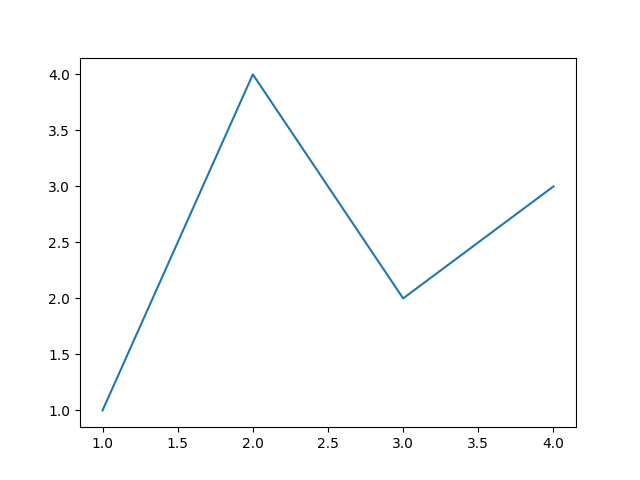
\includegraphics[width=0.8\textwidth]{figs/plot.png}
	\end{figure}
	\item A figura tem várias partes, onde cada uma pode ser alterada
	
	\begin{figure}[htb!]
		\centering
		\caption{Partes da figura no Matplotlib}
		\label{fig:anatomy}
		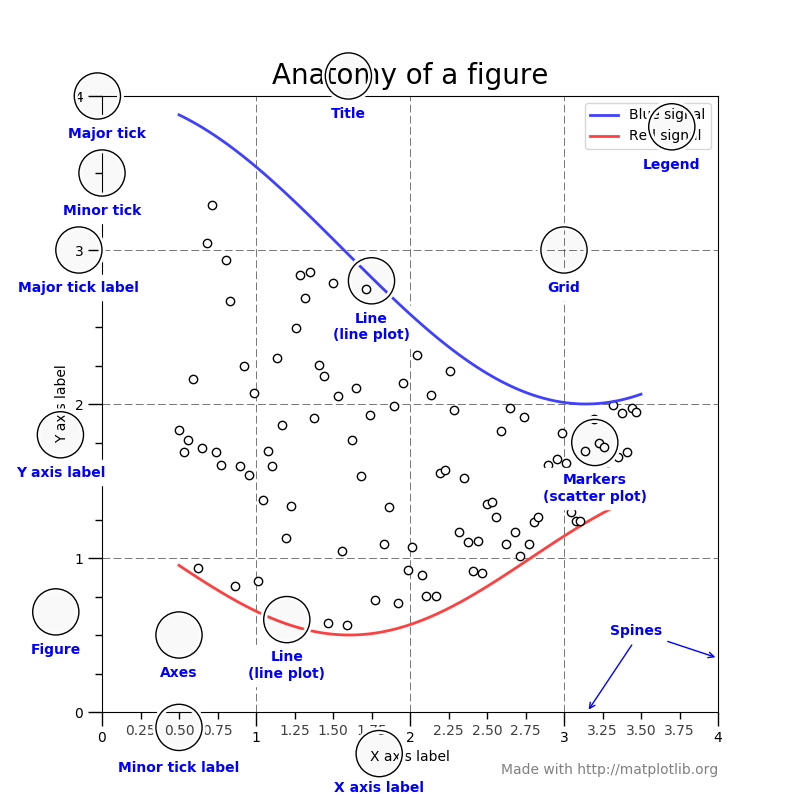
\includegraphics[width=0.8\textwidth]{figs/anatomy}\\
		\tiny{Fonte: Documentação do Matplotlib}
	\end{figure}
	
	\begin{description}
		\item[Figura (Figure)] A figura \textbf{toda}. Armazena os eixos, elementos "especiais" (títulos, legendas, etc). Cria-se usando o \textit{pyplot}:
		\begin{minted}{python}
fig = plt.figure()  # uma figura vazia sem eixos
fig, ax = plt.subplots()  # uma figura com um único eixo
fig, axs = plt.subplots(2, 2)  # uma figura com uma grade de eixos 2x2
		\end{minted}
		\item[Eixos (Axes)] O \textit{plot} de fato. É a região da imagem com os dados espaciais. Os \textit{Axes} podem ter dois (ou três no caso 3D) \textit{Axis}(ver abaixo) que lida com os limites do gráfico. Cada \textit{Axes} pode ter seu próprio título e legendas para x e y.
		\item[Eixo (Axis)] A linha numerada. Tem os limites do gráfico e os marcadores, bem como os nomes dos marcadores.
	\end{description}
	\item Tipos de gráficos comuns:
	\begin{description}
		\item[plot] Plota $x$ vs $y$ como linhas e/ou marcadores
		\begin{minted}{python}
>>> plot(x, y)        # plota x e y usado tipo padrão de linha e cor
>>> plot(x, y, 'bo')  # plota x e y usando círculos azuis como marcadores
>>> plot(y)           # plota y usando x como um vetor de 0 até N-1
>>> plot(y, 'r+')     # igual acima, mas com + vermelhos de marcador
		\end{minted}
		\item[stem] Plota linhas perpendiculares em relação à linha de base, começando na linha de base e terminando no topo, e coloca um marca nesse lugar. Normalmente, $x$ são as posiçoes e $y$ os topos.
		\begin{minted}{python}
x = np.linspace(0.1, 2 * np.pi, 41)
y = np.exp(np.sin(x))
plt.stem(x, y)
plt.show()
		\end{minted}
		
		\begin{figure}[htb!]
			\centering
			\caption{Stem}
			\label{fig:stem}
			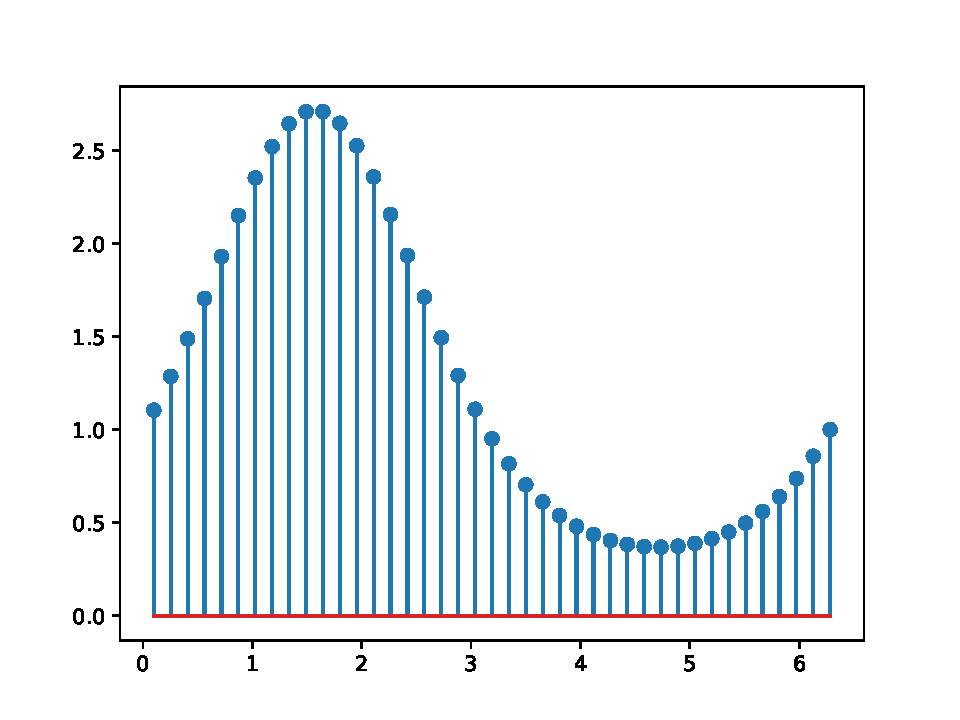
\includegraphics[width=0.8\textwidth]{figs/stem.pdf}
		\end{figure}
		\item[scatter] Plota y vs x com diferentes tamanhos e cores dos marcadores
		\begin{minted}{python}
# fixa a semente de números aleatórios
np.random.seed(19680801)

N = 50
x = np.random.rand(N)
y = np.random.rand(N)
colors = np.random.rand(N)
area = (30 * np.random.rand(N))**2  # 0 até 15 pontos o tamanho do raio

plt.scatter(x, y, s=area, c=colors, alpha=0.5)
plt.show()
		\end{minted}
		
		\begin{figure}[htb!]
			\centering
			\caption{Scatter}
			\label{fig:scatter}
			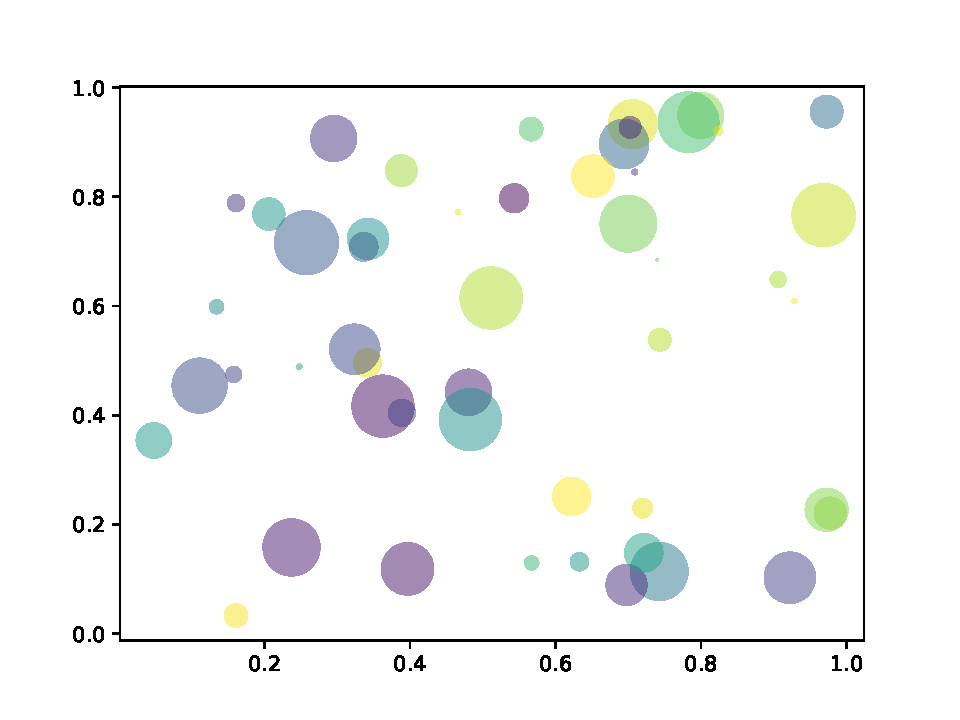
\includegraphics[width=0.8\textwidth]{figs/scatter.pdf}
		\end{figure}
	\end{description}
	\item Mais comandos e exemplos do \textit{Matplotlib} estão na \href{https://matplotlib.org/stable/contents.html}{documentação online} (em inglês)
\end{itemize}

\section{Dicas gerais}
\begin{itemize}
	\item Use 4 espaços para endentação, e não tabulações (alguns editores de texto convertem automaticamente as tabulações para 4 espaços, vale verificar)
	\item Nomeie as variáveis de acordo com o que elas se referem de maneira explícita (usar \verb|area| ao invés de \verb|a|, por exemplo)
	\item Nomeie variáveis e funções com letras minúsculas e palavras separadas por espaço (esse método é chamado de \verb|snake_case|)
	\item Escreva linhas com até 79 caracteres, e até 72 se for linha com comentário (a maioria dos editores de texto exibe o número de caracteres)
	\item Use linhas em branco para separar funções ou longos blocos de texto dentro de funções
	\item Quando possível, coloque o comentário na linha a que se refere (respeitando o limite de caracteres citado acima)
	\item Use \textit{docstrings} para arquivos e funções, descrevendo de maneira adequada o uso
	\item Use espaços entre operadores e depois de vírgulas (ex.: \verb|a = f(1, 2) + g(3, 4)|)
	\item Mais comandos e recursos do \textit{Python} podem ser encontrados no \href{https://docs.python.org/3/tutorial/index.html}{tutorial online} (em inglês), e dicas de estilo (como deixar o código "bonito" para o \textit{Python}) estão no documento chamado \href{https://www.python.org/dev/peps/pep-0008}{PEP 8} (em inglês)
\end{itemize}